% Options for packages loaded elsewhere
\PassOptionsToPackage{unicode}{hyperref}
\PassOptionsToPackage{hyphens}{url}
\PassOptionsToPackage{dvipsnames,svgnames,x11names}{xcolor}
%
\documentclass[
  a4paper,
  DIV=11,
  numbers=noendperiod]{scrreprt}

\usepackage{amsmath,amssymb}
\usepackage{iftex}
\ifPDFTeX
  \usepackage[T1]{fontenc}
  \usepackage[utf8]{inputenc}
  \usepackage{textcomp} % provide euro and other symbols
\else % if luatex or xetex
  \usepackage{unicode-math}
  \defaultfontfeatures{Scale=MatchLowercase}
  \defaultfontfeatures[\rmfamily]{Ligatures=TeX,Scale=1}
\fi
\usepackage{lmodern}
\ifPDFTeX\else  
    % xetex/luatex font selection
\fi
% Use upquote if available, for straight quotes in verbatim environments
\IfFileExists{upquote.sty}{\usepackage{upquote}}{}
\IfFileExists{microtype.sty}{% use microtype if available
  \usepackage[]{microtype}
  \UseMicrotypeSet[protrusion]{basicmath} % disable protrusion for tt fonts
}{}
\makeatletter
\@ifundefined{KOMAClassName}{% if non-KOMA class
  \IfFileExists{parskip.sty}{%
    \usepackage{parskip}
  }{% else
    \setlength{\parindent}{0pt}
    \setlength{\parskip}{6pt plus 2pt minus 1pt}}
}{% if KOMA class
  \KOMAoptions{parskip=half}}
\makeatother
\usepackage{xcolor}
\setlength{\emergencystretch}{3em} % prevent overfull lines
\setcounter{secnumdepth}{5}
% Make \paragraph and \subparagraph free-standing
\ifx\paragraph\undefined\else
  \let\oldparagraph\paragraph
  \renewcommand{\paragraph}[1]{\oldparagraph{#1}\mbox{}}
\fi
\ifx\subparagraph\undefined\else
  \let\oldsubparagraph\subparagraph
  \renewcommand{\subparagraph}[1]{\oldsubparagraph{#1}\mbox{}}
\fi


\providecommand{\tightlist}{%
  \setlength{\itemsep}{0pt}\setlength{\parskip}{0pt}}\usepackage{longtable,booktabs,array}
\usepackage{calc} % for calculating minipage widths
% Correct order of tables after \paragraph or \subparagraph
\usepackage{etoolbox}
\makeatletter
\patchcmd\longtable{\par}{\if@noskipsec\mbox{}\fi\par}{}{}
\makeatother
% Allow footnotes in longtable head/foot
\IfFileExists{footnotehyper.sty}{\usepackage{footnotehyper}}{\usepackage{footnote}}
\makesavenoteenv{longtable}
\usepackage{graphicx}
\makeatletter
\def\maxwidth{\ifdim\Gin@nat@width>\linewidth\linewidth\else\Gin@nat@width\fi}
\def\maxheight{\ifdim\Gin@nat@height>\textheight\textheight\else\Gin@nat@height\fi}
\makeatother
% Scale images if necessary, so that they will not overflow the page
% margins by default, and it is still possible to overwrite the defaults
% using explicit options in \includegraphics[width, height, ...]{}
\setkeys{Gin}{width=\maxwidth,height=\maxheight,keepaspectratio}
% Set default figure placement to htbp
\makeatletter
\def\fps@figure{htbp}
\makeatother
\newlength{\cslhangindent}
\setlength{\cslhangindent}{1.5em}
\newlength{\csllabelwidth}
\setlength{\csllabelwidth}{3em}
\newlength{\cslentryspacingunit} % times entry-spacing
\setlength{\cslentryspacingunit}{\parskip}
\newenvironment{CSLReferences}[2] % #1 hanging-ident, #2 entry spacing
 {% don't indent paragraphs
  \setlength{\parindent}{0pt}
  % turn on hanging indent if param 1 is 1
  \ifodd #1
  \let\oldpar\par
  \def\par{\hangindent=\cslhangindent\oldpar}
  \fi
  % set entry spacing
  \setlength{\parskip}{#2\cslentryspacingunit}
 }%
 {}
\usepackage{calc}
\newcommand{\CSLBlock}[1]{#1\hfill\break}
\newcommand{\CSLLeftMargin}[1]{\parbox[t]{\csllabelwidth}{#1}}
\newcommand{\CSLRightInline}[1]{\parbox[t]{\linewidth - \csllabelwidth}{#1}\break}
\newcommand{\CSLIndent}[1]{\hspace{\cslhangindent}#1}

\KOMAoption{captions}{tableheading}
\makeatletter
\makeatother
\makeatletter
\makeatother
\makeatletter
\@ifpackageloaded{caption}{}{\usepackage{caption}}
\AtBeginDocument{%
\ifdefined\contentsname
  \renewcommand*\contentsname{Table of contents}
\else
  \newcommand\contentsname{Table of contents}
\fi
\ifdefined\listfigurename
  \renewcommand*\listfigurename{List of Figures}
\else
  \newcommand\listfigurename{List of Figures}
\fi
\ifdefined\listtablename
  \renewcommand*\listtablename{List of Tables}
\else
  \newcommand\listtablename{List of Tables}
\fi
\ifdefined\figurename
  \renewcommand*\figurename{Figure}
\else
  \newcommand\figurename{Figure}
\fi
\ifdefined\tablename
  \renewcommand*\tablename{Table}
\else
  \newcommand\tablename{Table}
\fi
}
\@ifpackageloaded{float}{}{\usepackage{float}}
\floatstyle{ruled}
\@ifundefined{c@chapter}{\newfloat{codelisting}{h}{lop}}{\newfloat{codelisting}{h}{lop}[chapter]}
\floatname{codelisting}{Listing}
\newcommand*\listoflistings{\listof{codelisting}{List of Listings}}
\makeatother
\makeatletter
\@ifpackageloaded{caption}{}{\usepackage{caption}}
\@ifpackageloaded{subcaption}{}{\usepackage{subcaption}}
\makeatother
\makeatletter
\@ifpackageloaded{tcolorbox}{}{\usepackage[skins,breakable]{tcolorbox}}
\makeatother
\makeatletter
\@ifundefined{shadecolor}{\definecolor{shadecolor}{rgb}{.97, .97, .97}}
\makeatother
\makeatletter
\makeatother
\makeatletter
\makeatother
\ifLuaTeX
  \usepackage{selnolig}  % disable illegal ligatures
\fi
\IfFileExists{bookmark.sty}{\usepackage{bookmark}}{\usepackage{hyperref}}
\IfFileExists{xurl.sty}{\usepackage{xurl}}{} % add URL line breaks if available
\urlstyle{same} % disable monospaced font for URLs
\hypersetup{
  pdftitle={Who Counts as Australian?},
  pdfauthor={Kelly Tall; Michael Falk; Heather Ford; Tamson Pietsch},
  pdfkeywords={Wikipedia, historiography, Australia, digital
humanities, systemic bias},
  colorlinks=true,
  linkcolor={blue},
  filecolor={Maroon},
  citecolor={Blue},
  urlcolor={Blue},
  pdfcreator={LaTeX via pandoc}}

\title{Who Counts as Australian?}
\author{Kelly Tall \and Michael Falk \and Heather Ford \and Tamson
Pietsch}
\date{2023-11-08}

\begin{document}
\maketitle
\ifdefined\Shaded\renewenvironment{Shaded}{\begin{tcolorbox}[sharp corners, interior hidden, frame hidden, boxrule=0pt, breakable, borderline west={3pt}{0pt}{shadecolor}, enhanced]}{\end{tcolorbox}}\fi

\renewcommand*\contentsname{Table of contents}
{
\hypersetup{linkcolor=}
\setcounter{tocdepth}{2}
\tableofcontents
}
\textbf{Work in progress. Not for public distribution.}

\hypertarget{introduction}{%
\chapter{Introduction}\label{introduction}}

Who counts as Australian in Wikipedia and its sister-projects? How are
Wikipedia articles or Wikidata items marked as `Australian' by the
system? How does Wikipedia define or represent `Australianness'? In this
report, we try to address these questions using a dataset of
biographical articles culled from English Wikipedia. We have two primary
aims: (1) to reveal the definition of `Australianess' implicit in
Wikipedia's systems; (2) to assess how well Wikipedia represents the
diversity of Australians. As we will see, Wikipedia works implicitly
with numerous inconsistent definitions of `Australianness', but it is
nonetheless possible to make some reasonable observations about how well
it represents the diversity of people who make up `Australia'.

People can be represented in Wikipedia in many ways. They may have an
empty article that redirects to another article that concerns them
(e.g.~\href{https://en.wikipedia.org/wiki/Azaria_Chamberlain}{Azaria
Chamberlain}). They may be mentioned in the text of an article
(e.g.~Sasha Soldatow or the `manual workers' in
\href{https://en.wikipedia.org/w/index.php?title=Sydney_Push\&oldid=1151477281}{Sydney
Push}). Or they might have a full-blown article devoted to their
biography (e.g.~\href{https://en.wikipedia.org/wiki/Ada_Cambridge}{Ada
Cambridge}). For the sake of our analysis, we focus on the third kind of
representation: the biographical article. This allows us to quantify our
analysis, because each article in the dataset equals one person.

We explain how we construct the dataset in
\protect\hyperlink{data}{Data}. Broadly, we use two methods to identify
`Australian' biographies in Wikipedia. First, we use
\protect\hyperlink{wikipedias-category-system}{Wikipedia's category
system} to find all biographies contained in
\href{https://en.wikipedia.org/wiki/Category:Australian_people}{Category:Australian
people}. Second, we use
\protect\hyperlink{wikidatas-query-service}{Wikidata's query service} to
find all biographies whose corresponding Wikidata item has a property
suggestive of `Australianness' (e.g.~a
\href{https://www.wikidata.org/wiki/Property:P9159}{People Australia
ID}). Using these two methods, we identify 83,013 biographies on English
Wikipedia that are marked as `Australian' in some way. We enrich these
biographies with additional \protect\hyperlink{metadata}{Metadata} for
further analysis.

Our \protect\hyperlink{analysis}{Analysis} of the data unfolds in four
main sections. In \protect\hyperlink{australianness}{Australianness}, we
consider what it means for a person to be `Australian' in Wikipedia.
Where does the system draw the line(s) between Australians and
non-Australians? We show that the system draws many different lines,
which do not always conform with one another. In the subsequent sections
of analysis, we consider how Wikipedia captures the diversity of
Australia's people, along the axes of
\protect\hyperlink{gender}{Gender},
\protect\hyperlink{indigeneity}{Indigeneity} and
\protect\hyperlink{historical-period}{Historical period}. We demonstrate
that it is possible to make some generalisations about how Australians
are represented in Wikipedia. In particular, we observe considerable
normativity in the encyclopaedia: generally, Wikipedia assumes that an
`Australian' is a white cisgender male; only if a person departs from
this norm are their racial or sexual characteristics explicitly
described. While representation of some minority groups may be improving
(e.g.~the gap between Indigenous and settler Australians), other
representation gaps remain tenacious (e.g.~the gender gap).

In \protect\hyperlink{conclusion-beyond-bias}{Conclusion: beyond bias},
we make some suggestions about how Wikipedians might like to improve the
representation of Australians in the encyclopaedia. As well as
addressing the traditional problem of `systemic bias', we suggest that
Wikipedians draw attention to the \emph{representational multiplicity}
of Wikipedia, so that visitors and editors can become more aware of the
multiple definitions of `Australianness' across the Wikiverse.

\begin{figure}

{\centering 
\includegraphics{assets/objective-2.jpg}

}

\caption{How do Wikipedians construct Australia online?}

\end{figure}

\hypertarget{data}{%
\chapter{Data}\label{data}}

The code to generate this report is contained in two files in the
\href{https://github.com/wikihistories/reports}{wikihistories reports
Github repository}:

\begin{itemize}
\tightlist
\item
  \href{https://github.com/wikihistories/reports/tree/main/scripts/who-counts-lib.R}{who-counts-lib.R}
  contains all the functions to import the data
\item
  \href{https://github.com/wikihistories/reports/tree/main/scripts/who-counts-data.R}{who-counts-data.R}
  combines the functions to import the full dataset. This script can be
  run with \texttt{USE\_CACHE\ \textless{}-\ TRUE} to import the data
  from the saved files for this report, or
  \texttt{USE\_CACHE\ \textless{}-\ FALSE} to regenerate the data afresh
  from Wikipedia and Wikidata
\end{itemize}

All the source code for the analysis is included in this report, and can
be viewed on Github at
\href{https://github.com/wikihistories/reports/tree/main/who-counts.qmd}{who-counts.qmd}.

\hypertarget{wikipedias-category-system}{%
\section{Wikipedia's category system}\label{wikipedias-category-system}}

From its inception, Wikipedia has provided a category system to
`\href{https://en.wikipedia.org/w/index.php?title=Help:Category\&oldid=1174603713}{group
together pages on similar subjects}', and provide useful
`\href{https://en.wikipedia.org/w/index.php?title=Wikipedia:Categorization\&oldid=1181497476}{navigational
links to pages in Wikipedia}'. Wikipedia's categories form a vast and
complex tree. A category may contain infintely many subcategories, and
those subcategories may themselves belong to infinitely many
supercategories. Nearly all Wikipedia articles are categorised, partly
due to the work of a
\href{https://en.wikipedia.org/wiki/Wikipedia:WikiProject_Categories/uncategorized}{task
group and patrol} whose job is to hunt down any uncategorised articles.

In this context, the first place we looked for biographies of Australian
people on Wikipedia was
\href{https://en.wikipedia.org/wiki/Category:Australian_people}{Category:Australian
people}, which `lists notable Australian-born people, or people who
identify themselves as Australian'. This category contains 99,626
articles on English Wikipedia, and the number has grown consistently
(Figure~\ref{fig-included-in-ozpeople-over-time}).\footnote{The growth
  was calculated using the \texttt{timestamp} data returned by
  \href{https://www.mediawiki.org/wiki/API:Categorymembers}{API:Categorymembers}.
  The \texttt{timestamp} records when an article, file or subcategory
  was included in a given category. The documentation does not explain
  how the inclusion time is calculated for pages that are removed from
  and then re-included in a category. If an article was included in
  multiple subcategories of Category:Australian people, then the
  earliest timestamp was used to calculate its position in the figure.}

\begin{figure}

{\centering 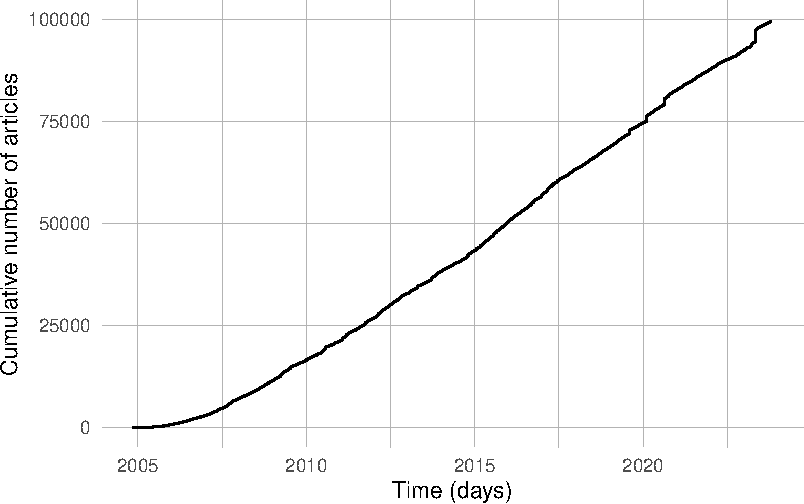
\includegraphics{who-counts_files/figure-pdf/fig-included-in-ozpeople-over-time-1.pdf}

}

\caption{\label{fig-included-in-ozpeople-over-time}Category:Australian
people has grown consistently since the early days of Wikipedia}

\end{figure}

Not all the articles in \texttt{Category:Australian\ people} are
biographies. In the first case, there are many articles about groups of
Australian people,
e.g.~\href{https://en.wikipedia.org/wiki/Aboriginal_Victorians}{Aboriginal
Victorians} or
\href{https://en.wikipedia.org/wiki/Australian_Chamber_Orchestra}{Australian
Chamber Orchestra}. In the second case,
\texttt{Category:Australian\ people} is a vast category, with 9,492
subcategories. In the trackless expanse of these subcategories, some
unexpected articles make their way into
\texttt{Category:Australian\ people}, such as the classic glam rock
album
\href{https://en.wikipedia.org/wiki/Living_in_the_70\%27s}{\emph{Living
in the '70s}}. We explain the `eccentricity' of the category graph when
we analyse Wikipedia's definition of
\protect\hyperlink{australianness}{Australianness} below. For now, we
simply describe our method for filtering all the non-biographies out of
\texttt{Category:Australian\ people}.

To filter out the non-biographies, we rely on Wikidata. We fetch the
Wikidata item for each article in \texttt{Category:Australian\ people},
and check to see if it has property
\href{https://www.wikidata.org/wiki/Property:P31}{P31}(\href{https://www.wikidata.org/wiki/Q5}{Q5}),
`instance of:human'. While the possession of P31(Q5) is not a perfect
signal that an article is a biography, we find that this criterion
filters out nearly all the non-biographies. Applying this criterion, we
identify 81,493 biographical articles in
\texttt{Category:Australian\ people}.

\hypertarget{wikidatas-query-service}{%
\section{Wikidata's query service}\label{wikidatas-query-service}}

Wikidata provides an alternative method for finding Australian
biographies: its \href{https://query.wikidata.org/}{query service}.
Using the query service, it is possible to search for Wikidata items
that possess given properties. If these Wikidata items have a
corresponding Wikipedia page, the link can be automatically retrieved.

It is more complex to find the `Australians' in Wikidata than in
Wikipedia. Wikipedia provides a single master-category for `Australian
people'. Wikidata does not. Instead, Wikidata can mark a person as
`Australian' in two main ways:

\begin{enumerate}
\def\labelenumi{\arabic{enumi}.}
\tightlist
\item
  It can explicitly link a person to Australia
  (\href{https://www.wikidata.org/wiki/Q408}{Q408}) through properties
  such as citizenship
  (\href{https://www.wikidata.org/wiki/Property:P27}{P27}), place of
  birth (\href{https://www.wikidata.org/wiki/Property:P19}{P19}) or
  place of death
  (\href{https://www.wikidata.org/wiki/Property:P570}{P570}); or
\item
  It can implicitly link a person to Australia by identifying them in a
  database of Australians, such as the Dictionary of Australian
  Biography
  (\href{https://www.wikidata.org/wiki/Property:P1907}{P1907}),
  Indigenous Australia
  (\href{https://www.wikidata.org/wiki/Property:P9246}{P9246}), or
  Convict Records of Australia
  (\href{https://www.wikidata.org/wiki/Property:P9919}{P9919})
\end{enumerate}

We queried Wikidata by 45 such properties suggesting Australianness.
Using these properties, we were able to identify 85,773 Wikidata items
representing Australian people. Of these Wikidata items, 63,692 items
had a corresponding Wikipedia article.

The two datasets overlap substantially, but not completely
(Figure~\ref{fig-biography-overlap-table}). There are thousands of
biographical articles in \texttt{Category:Australian\ people} whose
Wikidata items do not clearly identify them as `Australian'. Likewise,
there are hundreds of Wikidata items whose corresponding Wikipedia
articles do \emph{not} appear in \texttt{Category:Australian\ people},
even though the Wikidata item has P31(Q5), `instance of:human', and also
contains one or more `markers of Australianness'.

\begin{figure}

{\centering 

\begin{longtable}[]{@{}lr@{}}
\toprule\noalign{}
Dataset & Number of Articles \\
\midrule\noalign{}
\endhead
\bottomrule\noalign{}
\endlastfoot
Person only found by querying Wikidata & 1520 \\
Person only found in \texttt{Category:Australian\ people} & 19321 \\
Person found in both datasets & 62172 \\
\end{longtable}

}

\caption{\label{fig-biography-overlap-table}There is substantial, but
incomplete overlap between the biographies in the two datasets}

\end{figure}

\hypertarget{metadata}{%
\section{Metadata}\label{metadata}}

We combine our two datasets into a single larger dataset of 83,013
articles. To enable analysis of these articles, we then enrich them with
three kinds of metadata:

\begin{enumerate}
\def\labelenumi{\arabic{enumi}.}
\tightlist
\item
  Using the Wikidata Action API, we find each person's dates, birthplace
  and gender.
\item
  Using the Wikipedia Action API, we download the introduction of each
  article for text analysis.
\item
  Using the XTools API, we download page usage data for each page,
  including the page creation date, assessment class (e.g.~Good,
  Featured), pageviews and number of edits.
\end{enumerate}

\hypertarget{analysis}{%
\chapter{Analysis}\label{analysis}}

\hypertarget{australianness}{%
\section{Australianness}\label{australianness}}

In this report, we do not seek to define what it means to be
`Australian'. Instead, we aim to identify the `markers of
Australianness' that define what it means to be `Australian' in
Wikipedia. We have already introduced these markers in the
\protect\hyperlink{data}{Data} section. In Wikipedia, the primary marker
of Australianness is membership of \texttt{Category:Australian\ people}.
In Wikidata, no marker can be said to be primary, but the most frequent
in our dataset is
\href{https://www.wikidata.org/wiki/Property:P27}{P27}(\href{https://www.wikidata.org/wiki/Q408}{Q408}),
a property meaning that a person is a `citizen' of Australia. In both
cases, we will see that there is a sharp divide between the way
Wikipedians have defined the marker, and they way they have used it.

There are two reasons we refrain from defining `Australian' for
ourselves. In the first case, our opinion is not at all important---what
matters is Wikipedia's opinion. In the second case, it is exceptionally
difficult to define `Australian' in a non-arbitrary way. In two
dimensions, \textbf{space} and \textbf{time}, the concept of
`Australian' poses startling difficulties.

In \textbf{space}, it is difficult to judge whether a person is close
enough to Australia to count as Australian. At one end of the specturm
is someone who is born, lives and dies in Australia, such as
\href{https://en.wikipedia.org/wiki/Oodgeroo_Noonuccal}{Oodgeroo
Noonuccal}. There can be no dispute that such a person is Australian. At
the other end of the spectrum is someone who has only a passing cultural
or economic connection to Australia, such as
\href{https://en.wikipedia.org/wiki/Steve_Wozniak}{Steve Wozniak}, one
of the more surprising members of \texttt{Category:Australian\ people}.
Then there is the problem of the diaspora. Are the children of
Australians Australian, even if born overseas? If, like
\href{https://en.wikipedia.org/wiki/Rupert_Murdoch}{Rupert Murdoch}, you
leave Australia and renounce your citizenship, do you remain Australian?
There may be easy answers to these questions in specific contexts, for
example, when calculating a person's tax liability or entitlement to
vote, but in the context of an encyclopaedic project like Wikipedia,
they cannot be easily resolved.

In \textbf{time}, it is difficult to judge when in history it becomes
reasonable to describe someone as `Australian'. Humans first arrived in
Australia some 60,000 years ago, but they did not call the continent
`Australia'. The term `Terra Australis' (`Southern Land') was coined by
16th-century Europeans. At this time, `Terra Australis' was merely a
proposal, as no European had visited either Australia or Antarctica. In
the end, neither Australia nor Antarctica matched European expectations
about the `Southern Land', though Australia, being the first that
Europeans visited, acquired the name. New South Wales was invaded by the
British in 1788. The term `Australia' was substituted for `Terra
Australis' in 1813. The colonies of Australia federated into a single
Commonwealth in 1901. The resulting Commonwealth of Australia only
achieved full independence from Britain in 1988. The problem of time is
compounded by geology. In the course of Australia's human occuption, the
very landmass has altered considerably. Only 10,000 years ago, the
Australian mainland, Papua New Guinea and Tasmania formed a single
contiguous landmass that geologers call
\href{https://en.wikipedia.org/wiki/Sahul}{Sahul}. Are all the people
who occupied Sahul at any point in time `Australians'? Or can only
residents or citizens of the country `Australia' be so named? Like
space, time wreaks havoc on the category `Australian'.

The editors of Wikipedia and Wikidata grapple with both these problems.
The result is a kind of categorical anarchy, where different parts of
the system work with different concepts of `Australianess' and apply
different criteria of connection. It is for this reason that we talk of
`markers of Australianness' in Wikipedia. How do these markers work?

\hypertarget{in-the-category-system}{%
\subsection{In the category system}\label{in-the-category-system}}

The primary marker of Australianness in Wikipedia, as we have seen, is
membership of \texttt{Category:Australian\ people}. The category offers
\href{https://en.wikipedia.org/w/index.php?title=Category:Australian_people\&oldid=1148961840}{simple
criteria for membership}:

\begin{quote}
This
\href{https://en.wikipedia.org/w/index.php?title=Wikipedia:Categorization\&oldid=1181497476}{category}
lists notable
\href{https://en.wikipedia.org/wiki/Australia}{Australian}-born people,
or people who identify themselves as Australian.
\end{quote}

A user who clicks on the hyperlink `Australian' will be taken to the
Wikipedia page for Australia, which defines Australia as follows:

\begin{quote}
\textbf{Australia}, officially the \textbf{Commonwealth of Australia},
is a
\href{https://en.wikipedia.org/w/index.php?title=Sovereign_state\&oldid=1182523263}{sovereign
country} comprising the
\href{https://en.wikipedia.org/w/index.php?title=Mainland_Australia\&oldid=1179467610}{mainland}
of the
\href{https://en.wikipedia.org/w/index.php?title=Australia_(continent)\&oldid=1182388022}{Australian
continent}, the island of
\href{https://en.wikipedia.org/w/index.php?title=Tasmania\&oldid=1181384565}{Tasmania},
and numerous
\href{https://en.wikipedia.org/w/index.php?title=List_of_islands_of_Australia\&oldid=1174981257}{smaller
islands}.
\end{quote}

These definitions seem to offer a strong answer to the problems of space
and time. `Australia' is the `Commonwealth of Australia', the sovereign
state that has existed since 1901. In space, a person must be `born' in
Australia, or `identify themselves' as a member of the country. In time,
Australia is the Commonwealth of Australia, and so has only existed
since 1901.

The problem is, this explicit definition does not at all describe the
contents of \texttt{Category:Australian\ people}. In the spatial
dimension, the category includes living people such as
\href{https://en.wikipedia.org/w/index.php?title=Steve_Wozniak\&oldid=1182335281}{Steve
Wozniak} and
\href{https://en.wikipedia.org/w/index.php?title=Darrell_Duffie\&oldid=1168175801}{Darrell
Duffie} who were neither born in Australia nor identify themselves with
it. In the time dimension, the category includes many historical figures
who long predeceased the Commonwealth of Australia, such as
\href{https://en.wikipedia.org/w/index.php?title=Bennelong\&oldid=1182881508}{Bennelong},
\href{https://en.wikipedia.org/w/index.php?title=Mary_Reibey\&oldid=1182294588}{Mary
Reiby},
\href{https://en.wikipedia.org/w/index.php?title=Robert_Lowe\&oldid=1176772405}{Robert
Lowe} and
\href{https://en.wikipedia.org/w/index.php?title=Louisa_Atkinson\&oldid=1178386165}{Louisa
Atkinson}. Finally, it lists thousands of entities that aren't people,
such as
\href{https://en.wikipedia.org/w/index.php?title=First_Ever\&oldid=1177339020}{First
Ever}, the sportswear manufacturer, and
`\href{https://en.wikipedia.org/w/index.php?title=Hand_on_Your_Heart\&oldid=1181812572}{Hand
on Your Heart}', the 1989 single by Kylie Minogue. How has
\texttt{Category:Australian\ people} expanded to include so many pages
that contradict its own explicit definition?

The answer lies in the category's size. When editors include articles in
\texttt{Category:Australian\ people}, they do not necessarily do so
intentionally. Category:Australian people is the root node of a vast
category
\href{https://en.wikipedia.org/wiki/Graph_(discrete_mathematics)}{graph}.
The editor who categorised
\href{https://en.wikipedia.org/wiki/Steve_Wozniak}{Steve Wozniak} as a
\href{https://en.wikipedia.org/wiki/Category:Academic_staff_of_the_University_of_Technology_Sydney}{staff
member of the University of Technology Sydney} was probably unaware that
they were thereby categorising Wozniak as an `Australian person'. The
category for academic staff at UTS lies several layers deep in the
category graph, 4 steps away from the root
(Figure~\ref{fig-wozniak-distance-from-oz}). Perhaps an editor may
quibble that a person who works at UTS is not necessarily `from Sydney',
but in the present state of the category graph, there is no other way to
mark a staff member of UTS. The category graph is strictly hierarchical.
A subcategory cannot be removed from its parent category for the sake of
a single page.

\begin{figure}

{\centering 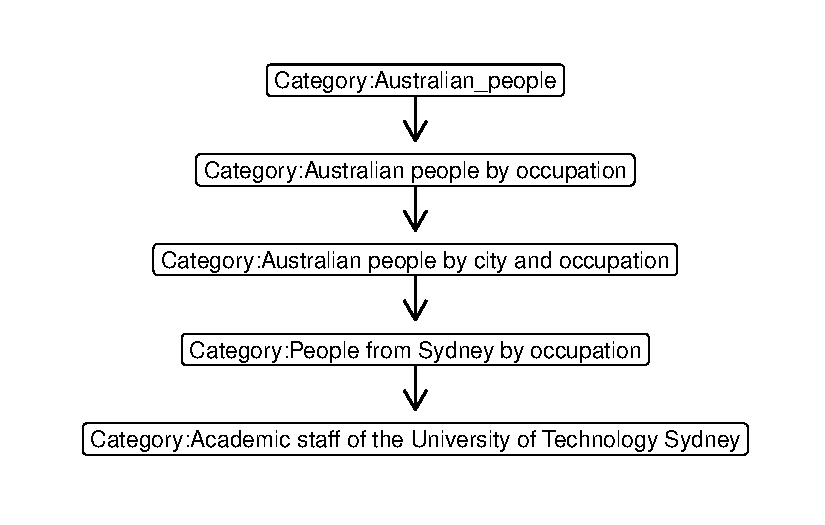
\includegraphics{who-counts_files/figure-pdf/fig-wozniak-distance-from-oz-1.pdf}

}

\caption{\label{fig-wozniak-distance-from-oz}The category for UTS staff
lies four steps away from Category:Australian people}

\end{figure}

Category:Australian people has 9,492 subcategories, many of which are
even farther from the root than the staff of UTS. We can get a sense of
how vast this structure is by taking
\href{https://en.wikipedia.org/wiki/Distance_(graph_theory)\#Related_concepts}{diameter}
of the category graph. In this case, the diameter is 11, which means
that the most distant subcategory of
\texttt{Category:Australian\ people} is 11 steps away. Such distant
nodes are called `eccentric' in graph theory. In this case, the most
distant subcategory truly is eccentric:
\href{https://en.wikipedia.org/wiki/Category:Custard\%20(band)\%20compilation\%20albums}{Category:Custard
(band) compilation albums} does not include articles about `Australian
people' at all, but about indie rock records. This case is extreme. The
case of UTS staffmembers is more typical. If we consider all the
articles that have been placed in \texttt{Category:Australian\ people}
or its subcategories, we find that the subcategories used are on average
3.17 steps away from the root, with a standard deviation of 0.95. In the
typical case, when an editor adds an article to an `Australian people'
subcategory, the subcategory is 2-4 steps away from the root. It seems
likely that editors are mostly unaware of the category graph as a whole.
Editors work locally, trying to find the best categorisations for their
articles, while Wikipedia's systems work globally, enforcing the
hierarchical logic of the enormous and usually invisible category graph.

There is thus a contradiction between the global and local logics of the
category graph. Frequently, the category graph also contradicts the
actual content of the encyclopaedia. First Ever is categorised as an
`Australian person' even though the text of the article identifies it as
`\href{https://en.wikipedia.org/w/index.php?title=First_Ever\&oldid=1177339020}{an
Australian manufacturing company}'.\footnote{In this case, the article
  falls under
  \href{https://en.wikipedia.org/w/index.php?title=Category:Clothing_brands_of_Australia\&oldid=938233678}{Category:Clothing
  brands of Australia}, which is a distant subcategory of
  \href{https://en.wikipedia.org/w/index.php?title=Category:Australian_designers\&oldid=921932361}{Category:Australian
  designers}, which is then linked through a number of other categories
  to
  \href{https://en.wikipedia.org/w/index.php?title=Category:Australian_people\&oldid=1148961840}{Category:Australian
  people}.} These contradictions breed a pervasive \emph{categorical
anarchy}. Seen from afar, Wikipedia is extremely lax about who or what
counts as `Australian'. A person---or even \emph{not} a person---can be
categorised as `Australian' for whatever reason seems reasonable in the
local context. Such laxity is probably necessary to Wikipedia's
encyclopaedic ambitions---how else could the vague concept of
`Australian person' ever find a place in Wikipedia? Wikidata is a
different beast. Rather than a collection of textual articles that can
speak for themselves, it is a database of structured facts (called
`claims') which are supposed to provide a reliable machine-readable
knowledge graph. Can categorical anarchy prevail in such a system?

\hypertarget{in-wikidata}{%
\subsection{In Wikidata}\label{in-wikidata}}

Wikidata's contributors are well aware of the difficulties of space and
time. The simplest way to mark someone as `Australian' in Wikidata is to
give `Australia' as the person's `country of citizenship'
(\href{https://www.wikidata.org/wiki/Property:P27}{P27}). Our dataset
contains 59,259 `Australian citizens' according to P27. A glance at
\href{https://www.wikidata.org/wiki/Property_talk:P27}{the Talk page for
P27} reveals that Wikidata's editors are well aware of the problems with
trying to categorised people as `Australian' in any stable way.

The user Ghouston clearly clearly articulates the problem of time in a
post from 2018:

\begin{quote}
It's not easy. Australian citizenship didn't exist before 1949, yet
Australia as a federation has existed since 1901 and the term
``Australian'' was in use in the 19th century. To say that the United
Kingdom was created in 1927 or the Netherlands perhaps in 1815 or 1945
or China in 1949 is to ignore much of the history of these countries as
states.
\end{quote}

Two years later, Ghouston provides additional sources and mentions a
possible solution:

\begin{quote}
Separate items for citizenships and nationalities have been proposed
previously. Perhaps it would help. The term ``Australian'' for people
living in Australia was already used in the 19th century, before
Australia had even been federated as a state, e.g.,
{[}\href{https://trove.nla.gov.au/newspaper/article/197054485}{2}{]}.
According to
{[}\href{https://www.passport-collector.com/evolution-australian-passport/}{3}{]},
Australia started issuing passports after federation, and didn't even
restrict it to British subjects until 1938, but it seems that passports
were not used much prior to WW1, and there was a more flexible attitude
to nationality.
\end{quote}

At the time of writing, there is
\href{https://www.wikidata.org/w/index.php?title=Wikidata:Property_proposal/Nationality\&oldid=1232071609}{no
Wikidata property for `nationality'}. Instead, the property of
citizenship is limited according to the `inception'
(\href{https://www.wikidata.org/wiki/Property:P571}{P571}) of the given
country and the death date of the given person. The start date of
Australia is given as \href{https://www.wikidata.org/wiki/Q408\#P571}{1
January 1901 in Wikidata}. If a person is assigned Australian
citizenship in Wikidata, and their death date occurs before 1 January
1901, then a warning appears in their Wikidata page. At the time of
writing,
\href{https://www.wikidata.org/w/index.php?title=Q1064745\&oldid=1933534532}{the
Wikidata item for colonial poet Charles Harpur} contains such a warning
(Figure~\ref{fig-citizenship-warning}). Harpur, who proudly described
himself as as `An Australian'
\href{http://nla.gov.au/nla.news-article32148201}{in newspaper
publications from the 1830s}, died in 1868.

\begin{figure}

{\centering 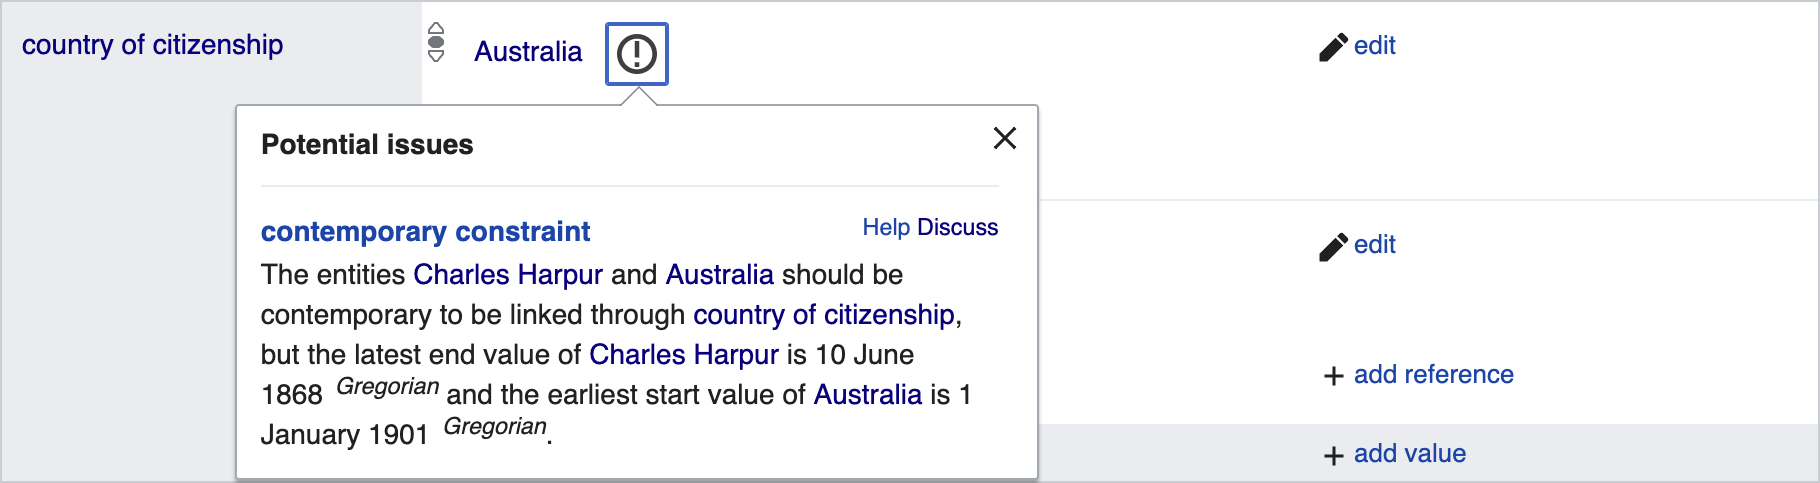
\includegraphics{assets/citizenship-warning.png}

}

\caption{\label{fig-citizenship-warning}Citzenship warning banner for
Charles Harpur}

\end{figure}

This solution combines flexibility with clarity.

\begin{itemize}
\tightlist
\item
  Flexibility: It is possible to mark the `Australianness' of Charles
  Harpur and others who have been identified as Australian throughout
  history.
\item
  Clarity: Wikidata provides clear guidance to its contributors through
  the warning banner. As far as Wikidata is concerned, Australian
  citizenship was available to people from 1901.
\end{itemize}

The price of this clarity and flexibility is inconsistency and
quixotism.

\begin{itemize}
\tightlist
\item
  Inconsistency: Wikidata flatly contradicts itself as far as historical
  figures like Charles Harpur are concerned. Was Harpur a citizen of
  Australia or not? Wikidata also contradicts, or at least brings into
  question, its own definition of `citizenship'. Wikidata defines
  citizenship (P27) thus:
  `\href{https://www.wikidata.org/wiki/Property:P27}{the object is a
  country that recognizes the subject as its citizen}' This definition
  is not reflected in P27's rules: all that is required is that the
  country exists prior to the supposed citizen's birth date. If Harpur
  were posthumously recognised as a citizen by the Commonwealth of
  Australia, this could not currently be reflected in the database. The
  warning banner would remain.
\item
  Quixotism: As Ghouston himself observes, Australia did not have an
  official system for conferring citizenship until 1949. By seeming to
  choose 1 January 1901 as earliest permitted date, Wikidata has
  invented its own concept of Australian citizenship. Is this quixotism
  consistent with Wikidata's self-description as a
  `\href{https://www.wikidata.org/wiki/Wikidata:Introduction}{secondary
  database, collecting structured data}'? Does Wikidata collect
  structured data, or does it structure collected data?
\end{itemize}

Wikimedians are aware of the difficulty of time. The state of P27
suggests that they are content for the minute to leave the difficulty
unresolved.

The difficulty of space is less clearly articulated on the talk page for
P27 (`country of citizenship'). Perhaps this is because the concept
`citizenship' presupposes a deep and publicly sanctioned connection
between the person and the country. In a sense, Wikidata delegates the
question of a person's spatial connection to Australia, by recording
when a person appears in a known database of Australians. These
databases make their own decisions about the `Australianness' of their
subjects. The Dictionary of Australian Biography, for example, does not
required its subjects to be Australian at all, as explained
\href{https://adb.anu.edu.au/faqs/\#aussie}{in their FAQs}:

\begin{quote}
\textbf{Do you have to be an Australian to be in the ADB?}\\
The ADB includes anyone who has made a significant contribution to the
Australian nation.
\end{quote}

The AusStage database, meanwhile,
\href{https://www.ausstage.edu.au/pages/learn/data-scope}{records any
person who `contributed' in some way to a theatrical performance in
Australia, or to an overseas performance of an Australian theatrical
work}. AusStage and the Australian Dictionary of Biography provide very
broad markers of Australianness. By contrast, the
\href{https://www.parliament.vic.gov.au/about/people-in-parliament/re-member/form/27}{Re-Member
database of the Parliament of Victoria} provides a stricter marker of a
person's Australianness. To appear in Re-Member, a person must be a
former member of the Parliament of Victoria. We identified dozens of
other databases that indicated `Australianess' in Wikidata. When a
Wikimedian links a person to the Australian Dictionary of Biography
(\href{https://www.wikidata.org/wiki/Property:P1907}{P1907}), AusStage
(\href{https://www.wikidata.org/wiki/Property:P8292}{P8292}), Re-Member
(\href{https://www.wikidata.org/wiki/Property:P8633}{P8633}), or some
other database of Australians, the linked database will encode a
different answer to the question `Who Counts as Australian?'

This raises the question: how do these different properties overlap in
Wikidata? Are there some markers of Australianness that tend to go
together? Are there others that exclude each other? For example, we
might assume that if a person is linked to the Convict Records of
Australia database
(\href{https://www.wikidata.org/wiki/Property:P9919}{P9919}), they
should not usually have Australia as their place of birth, since the
great majority of convicts were transported from Britain and Ireland,
rather than between the colonies.

To explore the connection between different markers of Australianness,
we generated a correlation plot between the 20 most common Wikidata
properties of the 45 that we queried
(Figure~\ref{fig-wikidata-property-matrix}). A red square indicates a
positive correlation between two Wikidata properties: for example, a
person with an
\href{https://www.wikidata.org/wiki/Property:P1907}{Australian
Dictionary of Biography ID} (\texttt{aus\_dictionary\_bio}) is highly
likely also to have a
\href{https://www.wikidata.org/wiki/Property:P9159}{People Australia ID}
(\texttt{people\_of\_aus}). A blue square indicates a negative
correlation between two properties: for example, a person marked as a
citizen of Australia is highly unlikely to have been assigned an
\href{https://www.wikidata.org/wiki/Property:P3546}{AustralianFootball.com
ID} (\texttt{aus\_football}).

\begin{figure}

{\centering 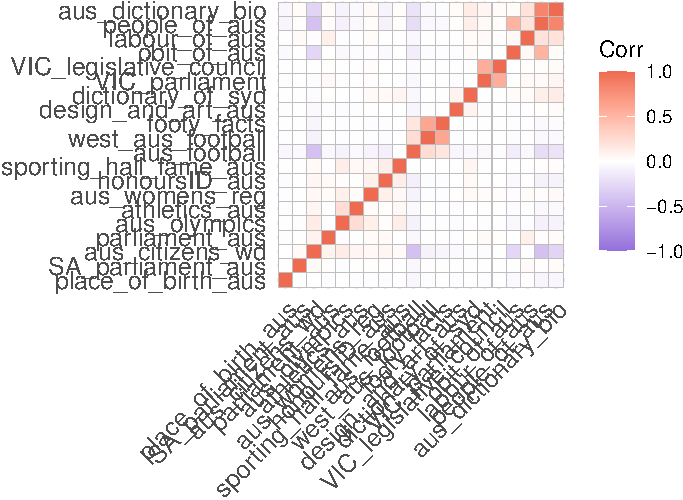
\includegraphics{who-counts_files/figure-pdf/fig-wikidata-property-matrix-1.pdf}

}

\caption{\label{fig-wikidata-property-matrix}Few of the properties are
strongly correlated}

\end{figure}

Only a few of the properties are correlated, and there are only a couple
of strong correlations in the matrix.

Many of the strong correlations reflect relationships between the
databases on which Wikidata relies for information. For example, it is
not surprising to see a strong correlation between Australian Dictionary
of Biography ID (\texttt{aus\_dictionary\_bio}), Labour Australia ID
(\texttt{labour\_of\_aus}), People Australia ID
(\texttt{people\_of\_aus}) and Obituaries of Australia ID
(\texttt{obit\_of\_aus}). These four databases are all run by the
National Centre for Biography at the Australian National University, and
are tightly interconnected. Every person in Obituaries Australia, Labour
Australia or the ADB automatically receives a People Australia ID.

Other strong correlations represent a similarity of subject-matter. For
instance, three Wikidata properties link to databases of Australian
artists (\texttt{nat\_gallery\_vic\_artist}, \texttt{aus\_printmakers},
\texttt{design\_and\_art\_aus}). A person who has an ID in one of these
external databases is likely to have an ID available in the others.
Similar explanations apply to sporting databases
(\texttt{atheltics\_aus} and \texttt{aus\_olympics}) and newspaper
databases (\texttt{obit\_of\_aus}).

Overall, the lack of correlation between the properties reflects the
heterogeneous nature of Wikidata. It is a vast and exceptionally
flexible database, and it is possible for different communities of
contributors to build up data in quite unrelated areas. This is
illustrated nowhere better than in the negative correlation between
AustralianFootball.com ID and the other Wikidata properties. Fans of
Australian Rules Football have painstakingly entered data about hundreds
of professional footballers into Wikidata, without troubling to mark
these records with other properties such as Trove ID or citizenship of
Australia. The shape of Wikidata could easily change if another
committed group of editors decided to document their own subculture in
the database. `Australian' is an extremely uneven and inconsistent idea
in Wikidata.

\hypertarget{gender}{%
\section{Gender}\label{gender}}

Although it is impossible to provide a unitary definition for
`Australian' in Wikidata and Wikipedia, we have shown that it is
possible to derive a large list of people who are marked as `Australian'
in some way across the encyclopaedia and database. What is the
composition of this list? We first consider the gendered composition of
the dataset, before turning to the representation of
\protect\hyperlink{indigeneity}{Indigenous Australians and Torres Strait
Islander peoples} in the next section.

To determine the gender of a person in our dataset, we rely on the
Wikidata property
\href{https://www.wikidata.org/wiki/Property:P21}{P21:Sex or gender}. In
our dataset, nearly all records have a sex or gender recorded
(Figure~\ref{fig-genders-in-dataset}). Only 2,065 records lack a
\texttt{P21} statement about their sex or gender.

\begin{figure}

{\centering 

\begin{longtable}[]{@{}lr@{}}
\toprule\noalign{}
Sex or Gender Label & Total \\
\midrule\noalign{}
\endhead
\bottomrule\noalign{}
\endlastfoot
faʻafafine & 1 \\
female & 23557 \\
genderfluid & 7 \\
genderqueer & 3 \\
intersex & 3 \\
intersex woman & 1 \\
male & 79386 \\
non-binary & 32 \\
trans man & 5 \\
trans woman & 31 \\
transgender & 2 \\
NA & 2065 \\
\end{longtable}

}

\caption{\label{fig-genders-in-dataset}There are many labels for
Australians' sex or gender across Wikimedia databases}

\end{figure}

Weathington and Brubaker (2023) have strongly critiqued Wikidata's
representation of sex and gender, observing that ``Queer identities are
recorded in a database in clunky, inaccurate, or self-contradictory
ways'' {[}p.~2{]} and that the database ignores the individual's right
to determine their own sexual presentation. Nonetheless, we are
compelled to rely on Wikidata's representation of individuals' sex
and/or gender if we wish to assess its representation of human diversity
in Australia. To this end, we categorise our dataset into three broad
groups: \texttt{Male}, \texttt{Female} and
\texttt{Trans,\ Non-Binary\ or\ Intersex}. While we may assume that most
of those marked as `male' or `female' are \emph{cis}-male or -female, we
cannot determine this from the available data, and so opt for the less
specific `male' and `female'.

\texttt{Female} biographies are clearly under-represented among
Wikipedia's Australian articles. (Figure~\ref{fig-genders-in-dataset})
shows all Wikipedia biographies that appear in
\texttt{Category:Australian\ people}, or whose Wikidata item contains a
marker of Australianness, categories by gender. The gap between
\texttt{Male} and \texttt{Female} biographies appears to have remained
constant over time (Figure~\ref{fig-gender-by-page-creation}). Viewing
the data on a logarithmic scale emphasise the parallel track of
\texttt{Male} and \texttt{Female} biographies in Australian Wikipedia,
while also allowing us to visualise the similar growth of
\texttt{Trans,\ Non-Binary\ or\ Intersex} biographies
(Figure~\ref{fig-gender-by-page-creation-log}).

\begin{figure}

{\centering 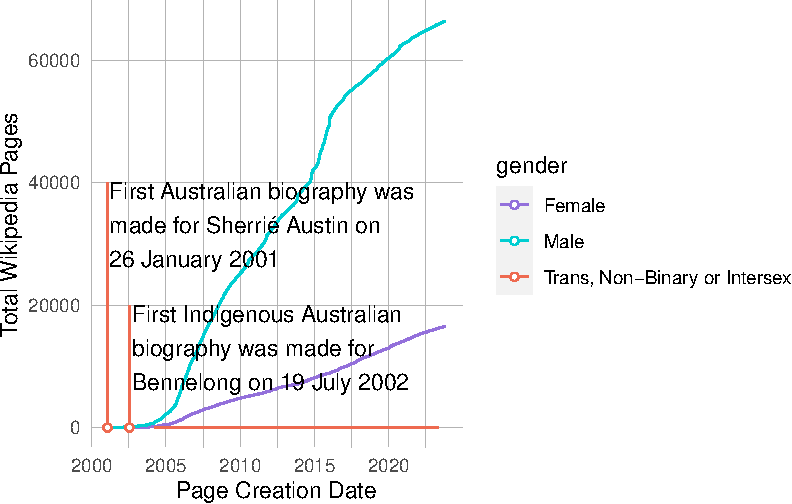
\includegraphics{who-counts_files/figure-pdf/fig-gender-by-page-creation-1.pdf}

}

\caption{\label{fig-gender-by-page-creation}Biographies of Australian
males continue to grow at least as fast as biographies of other
Australians.}

\end{figure}

\begin{figure}

{\centering 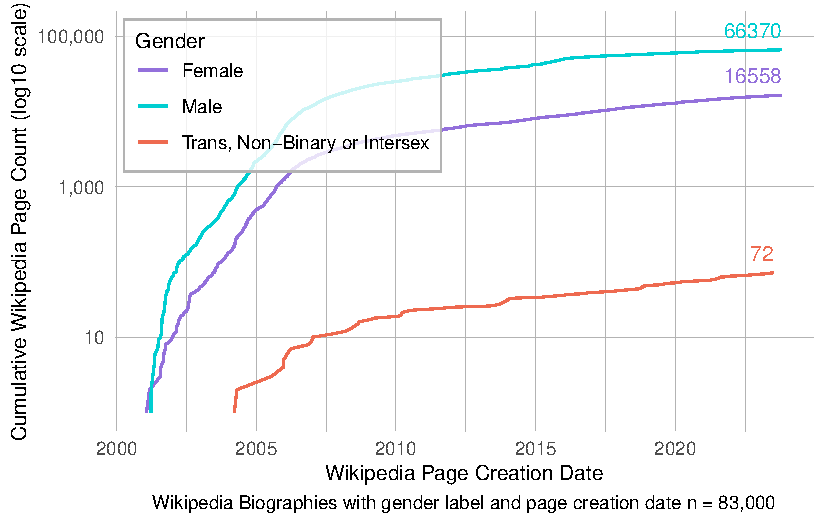
\includegraphics{who-counts_files/figure-pdf/fig-gender-by-page-creation-log-1.pdf}

}

\caption{\label{fig-gender-by-page-creation-log}It appears that
Australian biographies are growing equally quickly in all three gender
categories.}

\end{figure}

Not only are male, female and LGBTQI+ Australians represented in
different numbers in the encyclopaedia, they are represented by
different words. To show this, we downloaded the introductions of each
article in the encyclopaedia, and used the tf-idf statistic to determine
which words were most distinctive for each group of biographies. Which
words tend to appear more often in the introductions of articles about
\texttt{Male}, \texttt{Female} and
\texttt{Trans,\ Non-Binary\ and\ Intersex} Australians?

\begin{figure}

{\centering 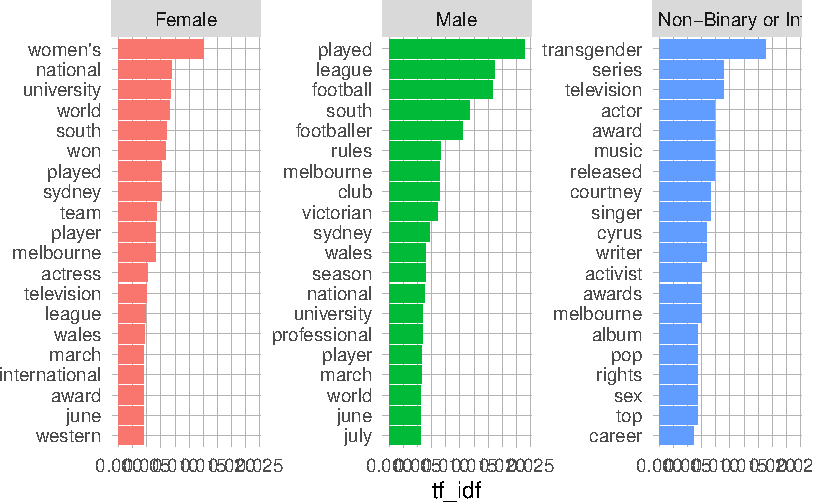
\includegraphics{who-counts_files/figure-pdf/fig-intro-words-by-gender-1.pdf}

}

\caption{\label{fig-intro-words-by-gender}Australian men's gender is
less explicitly marked in Wikipedia; non-Male Australians are more
likely to be activists and entertainers.}

\end{figure}

Figure~\ref{fig-intro-words-by-gender} discloses two significant
patterns:

\begin{itemize}
\tightlist
\item
  \emph{Explicit marking of non-Male genders}: First, Wikipedia articles
  are more likely to explicitly mention the sex or gender of a
  \texttt{Female} or \texttt{Trans,\ Non-Binary\ or\ Intersex}
  Australian. The high tf-idf score for ``women's'' in biographies of
  Females probably reflects the fact that female sporting teams are
  often have ``women's'' in their names. Thus Sam Kerr is said to
  represent Australian in the
  ``\href{https://en.wikipedia.org/w/index.php?title=Sam_Kerr\&oldid=1174642959}{national
  women's team}'', while Harry Kewell was simply a member of
  ``\href{https://en.wikipedia.org/w/index.php?title=Harry_Kewell\&oldid=1177164031}{the
  Australian national team}''. The situation for
  \texttt{Trans,\ Non-Binary\ and\ Intersex} Australians is even more
  marked. `Transgender', `sex' and `woman' all appear as distinctive
  terms in the introductions of Wikipedia biographies in this group.
\item
  \emph{Dominance of sport and entertainment}: Across all three gender
  categories, sport and entertainment are dominant themes. The
  \texttt{Male} biographies seem less likely to describe entertainers
  than those in the other categories. Unsuprisingly, the
  \texttt{Trans,\ Non-Binary\ and\ Intersex} biographies seem more
  likely to discuss social affairs, `activist' and `rights' being
  prominent terms in the introductions of these biographies.
\end{itemize}

The data support the views of Weathington and Brubaker (2023). In
Australian Wikipedia, maleness is the unmarked default. \texttt{Female}
and especially \texttt{Trans,\ Non-Binary\ and\ Intersex} Australians
are described using terms such as `women' or `transgender'; there is no
need to explicitly mention that a person is male or cisgender. In the
case of \texttt{Trans,\ Non-Binary\ and\ Intersex} people, this explicit
marking of gender goes a step further. Australians in this group are
likely to be described as `activists', presumbly on gender issues.
Biographies of \texttt{Trans,\ Non-Binary\ and\ Intersex} Australians
problematise gender in a manner that biographies of of \texttt{Male}
Australians do not.

Wikipedia's defaulting to malenes probably reflects the linguistic
habits of broader Australian society, but it could also be exacerbated
by the encylopaedia's obsession with sport and entertainment. Both sport
and entertainment are highly gendered fields. Men and women compete in
gendered competitions such as the soccer or cricket World Cups and
receive gendered commendations such as Best Actress at the Academy
Awards. While \texttt{Male} Australians may dominate non-\texttt{Male}
Australians in fields such as politics, business and the arts, these
fields are no so explicitly gendered. Sam Kerr may indeed be captain of
the ``women's national team,'' but it makes no sense to describe
\href{https://en.wikipedia.org/wiki/Vanessa_Hudson_(executive)}{Vanessa
Hudson} as the CEO of a ``women's corporation.'' Sport and entertainment
are fields that reflect society's deepest-held and most immoveable
convictions. Wikipedia's powerful focus on these fields may place the
encyclopaedia behind other parts of Australia in the evolution of
non-gendered language.

Finally in this section, we consider the attention received by
biographies in these three groups. Which Australians are the focus of
editor activity, and which are of most interest to readers? We used the
XTools API to download page usage statistics for articles in each group.
Figure~\ref{fig-assessment-data-by-gender} gives a snapshot of this
information.

\begin{figure}

{\centering 

\begin{longtable}[]{@{}
  >{\raggedright\arraybackslash}p{(\columnwidth - 14\tabcolsep) * \real{0.2190}}
  >{\raggedright\arraybackslash}p{(\columnwidth - 14\tabcolsep) * \real{0.0438}}
  >{\raggedright\arraybackslash}p{(\columnwidth - 14\tabcolsep) * \real{0.1241}}
  >{\raggedright\arraybackslash}p{(\columnwidth - 14\tabcolsep) * \real{0.1241}}
  >{\raggedright\arraybackslash}p{(\columnwidth - 14\tabcolsep) * \real{0.1095}}
  >{\raggedright\arraybackslash}p{(\columnwidth - 14\tabcolsep) * \real{0.1168}}
  >{\raggedright\arraybackslash}p{(\columnwidth - 14\tabcolsep) * \real{0.1606}}
  >{\raggedright\arraybackslash}p{(\columnwidth - 14\tabcolsep) * \real{0.1022}}@{}}
\toprule\noalign{}
\begin{minipage}[b]{\linewidth}\raggedright
gender
\end{minipage} & \begin{minipage}[b]{\linewidth}\raggedright
n
\end{minipage} & \begin{minipage}[b]{\linewidth}\raggedright
Pageviews (mean)
\end{minipage} & \begin{minipage}[b]{\linewidth}\raggedright
Revisions (mean)
\end{minipage} & \begin{minipage}[b]{\linewidth}\raggedright
Editors (mean)
\end{minipage} & \begin{minipage}[b]{\linewidth}\raggedright
Watchers (mean)
\end{minipage} & \begin{minipage}[b]{\linewidth}\raggedright
Weeks since last edit
\end{minipage} & \begin{minipage}[b]{\linewidth}\raggedright
Good/Featured
\end{minipage} \\
\midrule\noalign{}
\endhead
\bottomrule\noalign{}
\endlastfoot
Trans, Non-Binary or Intersex & 69 & 13644.7 & 424.6 & 164.2 & 37.2 &
8.5 & 1.4\% \\
Female & 16560 & 1391.2 & 105.5 & 49.9 & 2.8 & 22.7 & 0.6\% \\
Male & 66375 & 882.8 & 103.2 & 49.5 & 2.1 & 31.5 & 0.6\% \\
\end{longtable}

}

\caption{\label{fig-assessment-data-by-gender}Editors and readers of
Wikipedia appear to have different priorities when it comes to gender}

\end{figure}

Figure~\ref{fig-assessment-data-by-gender} reveals a stark contrast
between readers and editors of the encylopaedia. Editors spend roughly
equal effort on the \texttt{Male} and \texttt{Female} biographies. The
number of revisions for each biography, the number of editors, and the
time elapsed since last edit are all similar. The result is that
Wikipedia's editors expend a roughly 4 times the effort maintaining
\texttt{Male} biographies on Wikipedia than \texttt{Female} ones.
Readers of the encyclopaedia, however, have different priorities.
Although view biographies of \texttt{Male} Australians more often than
\texttt{Female}, an individual \texttt{Female} biography can expect to
be viewed roughly 1.6 times more often than any given biography of a
\texttt{Male} Australian.

Biographies of \texttt{Trans,\ Non-Binary\ or\ Intersex} Australians,
meanwhile, receive a great deal of attention from both editors and
readers compared to biographies in the other groups. Given there are
only 69 biographies in this group, the numbers are difficult to compare.
Editors probably pay extra attention to these pages because they are
more prone to vandalism by internet trolls. There would likely be
subsets of the \texttt{Male} and \texttt{Female} pages at risk of
similar vandalism, which would have a similar pageview and edit profile.
It is nonetheless sadly predictable that biographies of
\texttt{Trans,\ Non-Binary\ or\ Intersex} Australians should have such
high page activity on Wikipedia today.

In conclusion, it seems that the gender gap on Australian Wikipedia is
wide, and is not currently narrowing. Despite the under-representation
of women in the encyclopaedia, editors appear to devote equal attentions
both to \texttt{Male} and \texttt{Female} biographies. The number of
non-cisgender biographies appears to be very small---though it is
possible that many non-cisgender Australians have fallen into the
\texttt{Male} and \texttt{Female} groups in our analysis due to the
crude categorisation method. This small group of non-cisgender
biographies receieve a great deal of attention. The most likely reason
would appear to be vandalism, though we have not investigated this
hypothesis. Wikipedia appears to reflect aspects of Australian gender
culture, though the gender gap is probably inflated by the
encyclopaedia's strong focus on sport and entertainment, which are
highly gendered even by comparison to other fields of social endeavour.
This gender gap is reflected in the encyclopaedia's language as well as
in the sheer number of articles and editors' activities upon them. It
appears likely that Wikipedia is behind Australian society generally in
its representation of women, given that biographies of \texttt{Female}
Australians are so much more likely to be viewed than \texttt{Male}
biographies. If more \texttt{Female} Australians were represented in the
encylopaedia, would this ratio change? If the number of \texttt{Male}
and \texttt{Female} articles were equal, would readers still prefer to
read \texttt{Female} Australians' biographies, or would their average
interest decline as the total increased? At this point, we can only
speculate.

\hypertarget{indigeneity}{%
\section{Indigeneity}\label{indigeneity}}

The distinction between `settler' and `indigenous' Australian pervades
Wikipedia in a cryptic way. Race and ethncity are portrayed in a
lopsided manner in Wikipedia, much like gender. In English Wikipedia,
Mandiberg (2023) observes, people are not officially classified by
`race', but whiteness is assumed as a default, and a person is far more
likely to be categorised by their ethnic or national origin if they are
non-white.

There is no explicit category for `settler' or `white' Australian. There
are categories for
\href{https://en.wikipedia.org/wiki/Category:Immigrants_to_Australia}{Category:Immigrants
to Australia} and
\href{https://en.wikipedia.org/wiki/Category:Australian_people_of_European_descent}{Category:Australian
people of European Descent}, but these are applied only haphazardly to
indicate the `settler' status of a minority of Australians. A good
example is
\href{https://en.wikipedia.org/w/index.php?title=Tony_Abbott\&oldid=1178396384}{Tony
Abbott}. According to his Wikipedia biography, he was born in London to
English parents, and `migrated to Australia at the age of two'.
\href{https://en.wikipedia.org/w/index.php?title=Tony_Abbott\&action=info}{His
page is nearly 20 years old, and has been edited more than 4000 times.}.
Nonetheless, no-one has thought to categorise him either as an
`immigrant' or as an Australian `of European descent'. Extending
Mandiberg's arguments, we can hypothesise that `settler' status is
assumed in Australian Wikipedia, and a person's whiteness or migrant
status is considered unremarkable if they are British. We substantiate
this hypothesis below.

There may be no single category for `settler' or `white' Australian, but
there is certainly a single overarching category for
\href{https://en.wikipedia.org/w/index.php?title=Category:Indigenous_Australian_people\&oldid=971541573}{Indigenous
Australian people}. Within this category, editors are instructed to
sub-categorise Aboriginal and Torres Strait Islander Australians as
precisely as possible (Figure~\ref{fig-template-catdiffuse-indig-aus}).
These subcategories fall into three main kinds:

\begin{enumerate}
\def\labelenumi{\arabic{enumi}.}
\tightlist
\item
  Sub-categories for mob or language group,
  e.g.~\href{https://en.wikipedia.org/w/index.php?title=Category:Pitjantjatjara_people\&oldid=1141634439}{Category:Pitjantjatjara
  people}.
\item
  Sub-categories for occupation,
  e.g.~\href{https://en.wikipedia.org/w/index.php?title=Category:Indigenous_Australian_linguists\&oldid=1139800186}{Category:Indigenous
  Australian linguists} (Curiously, neither
  \href{https://en.wikipedia.org/w/index.php?title=Category:Australian_Aboriginal_guides\&action=info}{guide}
  nor
  \href{https://en.wikipedia.org/w/index.php?title=Category:Australian_Aboriginal_trackers\&oldid=1141656309}{tracker}
  is considered an occupation in this scheme.)
\item
  Miscellaneous subcategories, including
  \href{https://en.wikipedia.org/w/index.php?title=Category:Members_of_the_Stolen_Generations\&oldid=825612121}{Category:Members
  of the Stolen Generations},
  \href{https://en.wikipedia.org/w/index.php?title=Category:Last_known_speakers_of_an_Australian_Aboriginal_language\&oldid=951554350}{Category:Last
  known speakers of an Aboriginal language},
  \href{https://en.wikipedia.org/wiki/Category:Indigenous_Australian_feminists}{Category:Indigenous
  Australian feminists} and
  \href{https://en.wikipedia.org/w/index.php?title=Category:Australian_Aboriginal_elders\&oldid=940594168}{Category:Australian
  Aboriginal elders}.
\end{enumerate}

\begin{figure}

{\centering 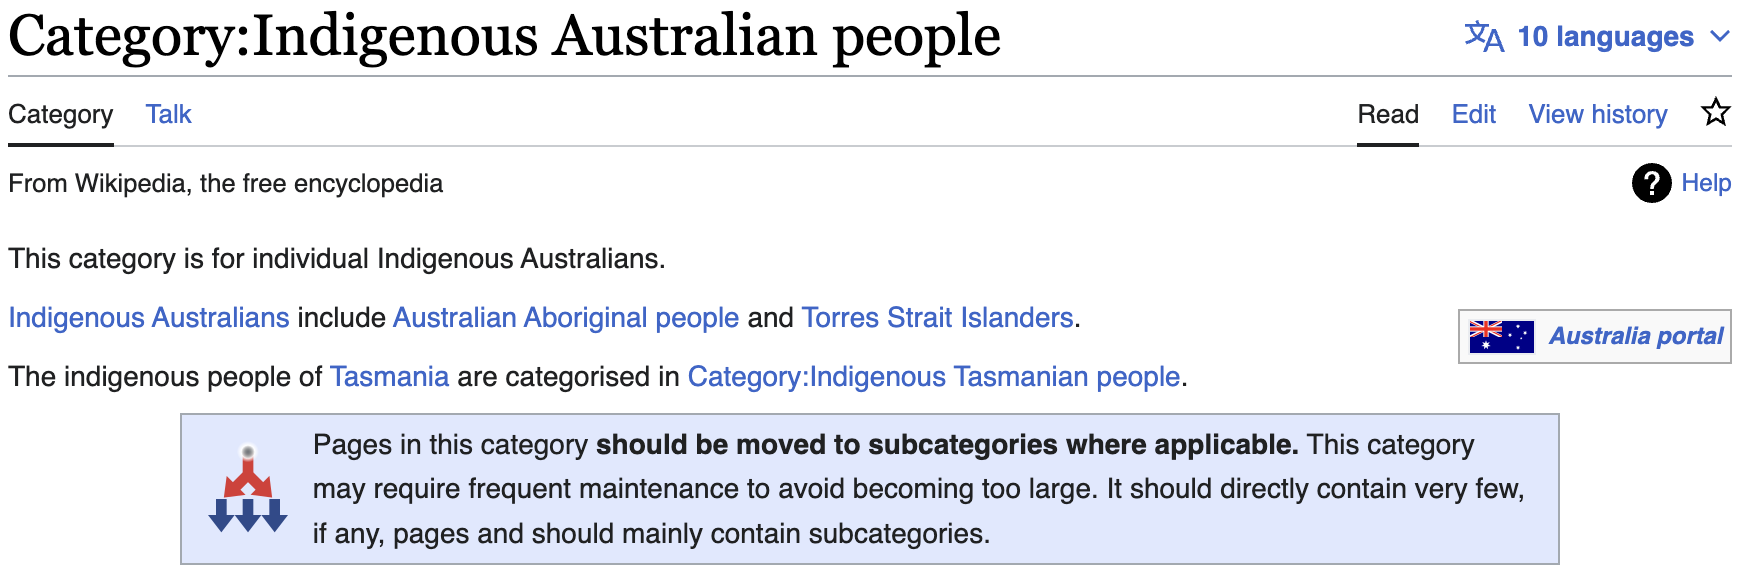
\includegraphics{assets/template-catdiffuse-indig-aus.png}

}

\caption{\label{fig-template-catdiffuse-indig-aus}\texttt{Template:Category\ diffuse}
instructs editors to categorise Indigenous Australian People more
precisely}

\end{figure}

\texttt{Category:Indigenous\ Australian\ people} is actually nested
quite deeply within the Australian category graph
(Figure~\ref{fig-ethnic-categorisation-graph}).
Figure~\ref{fig-ethnic-categorisation-graph} may at first be confusing
to Australian readers, because it is common in Australia to refer to
Aboriginal and Torres Strait Islander people as ``First Nations
Australians.'' In English Wikipedia's category graph, however, the term
``First Nations'' is used
\href{https://en.wikipedia.org/wiki/First_Nations_in_Canada}{the
Canadian sense}.\footnote{This has the notable corollary that there are
  no categories in Wikipedia for
  \href{https://en.wikipedia.org/wiki/M\%C3\%A9tis}{Métis} or
  \href{https://en.wikipedia.org/wiki/Inuit}{Inuit} Australians.} In
this instance, Wikipedia's category graph is potentially incendiary,
because it appears to imply there is no special connection between
Indigenous Australians and the continent to which they are indigenous.
The overarching
\texttt{Category:Australian\ people\ by\ ethnic\ or\ national\ origin}
is organised predominantly by continent or region. There are
sub-categories for Australians of
\href{https://en.wikipedia.org/wiki/Category:Australian_people_of_African_descent}{African},
\href{https://en.wikipedia.org/wiki/Category:Australian_people_of_Asian_descent}{Asian},
\href{https://en.wikipedia.org/wiki/Category:Australian_people_of_Caribbean_descent}{Carribean},
\href{https://en.wikipedia.org/wiki/Category:Australian_people_of_Latin_American_descent}{Latin
American},
\href{https://en.wikipedia.org/wiki/Category:Australian_people_of_Middle_Eastern_descent}{Middle
Eastern},
\href{https://en.wikipedia.org/wiki/Category:Australian_people_of_North_American_descent}{North
American} and
\href{https://en.wikipedia.org/wiki/Category:Australian_people_of_Oceanian_descent}{Oceanian}
descent. There is no category for ``Australians of Australian descent'',
nor is
\texttt{Category:Australian\ people\ of\ Indigenous\ Australian\ descent}
included as a subcategory of
\href{https://en.wikipedia.org/w/index.php?title=Category:Australian_people_of_Oceanian_descent\&oldid=607565632}{\texttt{Category:Australian\ people\ of\ Oceanian\ descent}}.\footnote{In
  other parts of English Wikipedia, Australia is included as part of
  Oceania. For instance,
  \texttt{Category:British\ people\ of\ Australian\ descent} is a
  subcategory of
  \texttt{Category:British\ people\ of\ Oceanian\ descent}. The same
  holds true for
  \href{https://en.wikipedia.org/wiki/Category:American_people_of_Oceanian_descent}{American},
  \href{https://en.wikipedia.org/wiki/Category:French_people_of_Oceanian_descent}{French},
  and
  \href{https://en.wikipedia.org/wiki/Category:Indian_people_of_Oceanian_descent}{Indian}
  people of Australian descent.} By contrast,
\texttt{Category:Australians\ of\ First\ Nations\ descent} is included
as a subcategory of
\href{https://en.wikipedia.org/w/index.php?title=Category:Australian_people_of_Canadian_descent\&oldid=649754186}{\texttt{Category:Australian\ people\ of\ Canadian\ descent}},
which is itself a subcategory of
\href{https://en.wikipedia.org/w/index.php?title=Category:Australian_people_of_North_American_descent\&oldid=839030224}{\texttt{Category:Australians\ of\ North\ American\ descent}}.
In this local portion of the graph, the link between First Nations
Canadians and Canada is formally encoded. The link between Indigenous
Australian people and Australia is not. A naïve reader of the graph
(such as a computer program) might erroneously conclude that
\texttt{First\ Nations} Australians have the same relationship to
Australia as \texttt{Indigenous} Australians.

\begin{figure}

{\centering 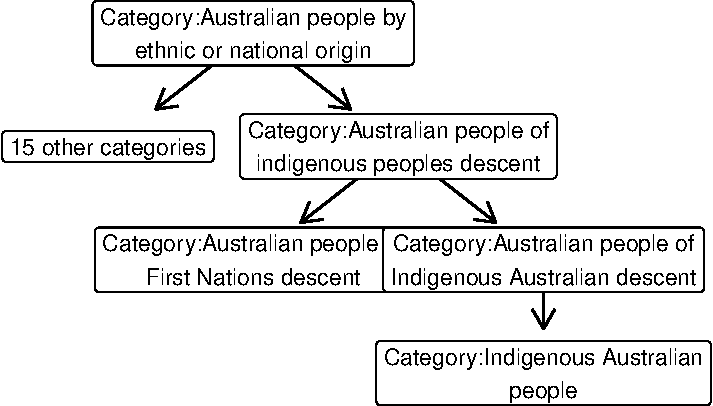
\includegraphics{who-counts_files/figure-pdf/fig-ethnic-categorisation-graph-1.pdf}

}

\caption{\label{fig-ethnic-categorisation-graph}Wikipedia has a complex,
settler-oriented method for categorising Australians by ethnic or
national origin}

\end{figure}

In Wikipedia's defence, the indigeneity of Indigenous Australians is
encoded in other ways. In this local portion of the graph, a human can
see from the \emph{labels} of
\texttt{Category:Australian\ people\ of\ Indigenous\ Australian\ descent}
and \texttt{Category:Indigenous\ Australian\ people} that people in
these categories are indigenous \emph{to Australia}. Looking beyond this
local portion of the graph, we can also see that
\href{https://en.wikipedia.org/wiki/Category:Indigenous_peoples_of_Australia}{\texttt{Category:Indigenous\ peoples\ of\ Australia}}
is a subcategory of
\href{https://en.wikipedia.org/wiki/Category:Indigenous_peoples_of_Oceania}{\texttt{Category:Indigenous\ peoples\ of\ Oceania}}.
It is nonetheless curious that the local portion of the graph that
classifies Australians by `ethnic or national origin' should
de-emphasise \texttt{Category:Indigenous\ Australian\ people}.

The situation is different for other countries in English Wikipedia.
Other settler-colonial countries include categories for their own
indigenous peoples directly beneath the super-category for
\texttt{people\ by\ ethnic\ or\ national\ origin}. For example,
\href{https://en.wikipedia.org/w/index.php?title=Category:Indigenous_Mexicans\&oldid=887057212}{Category:Indigenous
Mexicans} is a direct subcategory of
\href{https://en.wikipedia.org/w/index.php?title=Category:Mexican_people_by_ethnic_or_national_origin\&oldid=645962797}{Category:Mexican
people by ethnic or national origin}, while the analogous Australian
category, \texttt{Category:Indigenous\ Australian\ people}, is two steps
deeper in the graph. A similar pattern holds for other settler-colonial
states.
\href{https://en.wikipedia.org/wiki/Category:New_Zealand_people_by_ethnic_or_national_origin}{New
Zealand},
\href{https://en.wikipedia.org/wiki/Category:New_Caledonian_people_by_ethnic_or_national_origin}{New
Caledonia},
\href{https://en.wikipedia.org/wiki/Category:South_African_people_by_ethnic_or_national_origin}{South
Africa} and the
\href{https://en.wikipedia.org/wiki/Category:American_people_by_ethnic_or_national_origin}{United
States} all include top-level categories for their Indigenous peoples
under the \texttt{people\ by\ ethnic\ or\ national\ origin}
super-category.

There is a second notable difference between the category graphs for
Australia and Mexico. We have seen that Australia's
\texttt{Category:Australian\ people\ of\ indigenous\ peoples\ descent}
is used to classify people who are indigenous anywhere. The analogous
Mexican category,
\href{https://en.wikipedia.org/w/index.php?title=Category:Mexican_people_of_indigenous_peoples_descent\&oldid=812065156}{\texttt{Category:Mexican\ people\ of\ indigenous\ peoples\ descent}},
is used exclusively to classify indigenous peoples of Mexico itself.
\href{https://en.wikipedia.org/wiki/Category:Brazilian_people_by_ethnic_or_national_origin}{Brazil}
and
\href{https://en.wikipedia.org/wiki/Category:Brazilian_people_by_ethnic_or_national_origin}{Argentina}
similarly reserve their `indigenous peoples' category for their own
indigenous peoples.

Australia is not entirely alone. The subgraph for
\href{https://en.wikipedia.org/wiki/Category:Japanese_people_by_ethnic_or_national_origin}{\texttt{Category:Japanese\ people\ by\ ethnic\ or\ national\ origin}}
also obfuscates the indigeneity of Japan's indigenous peoples. There is
no explicit category for Japanese people `of indigenous descent'.
Instead,
\href{https://en.wikipedia.org/wiki/Category:Japanese_Ainu_people}{\texttt{Category:Japanese\ Ainu\ people}}
is included as a subcategory of
\href{https://en.wikipedia.org/wiki/Category:Japanese_people_of_East_Asian_descent}{\texttt{Category:Japanese\ people\ of\ East\ Asian\ descent}}.
In this way, the link between Ainu people and the region is locally
marked in the category graph, but one must look elsewhere in the graph
to discover that Ainu people are \emph{indigenous} to Japan.

It is clear that quantifying indigenous representation in Wikipedia is a
fraught exercise. Scholars are well advised to carefully consider how
indigeneity is understood in different parts of the world, and then to
pay close attention to the particular structure of ethnic and national
classification in any particular part of Wikipedia.

Nonetheless, we can use the category graph to estimate the number of
biographies of Indigenous Australians in Wikipedia.
Figure~\ref{fig-indigenous-growth-wikipedia} suggests that in recent
years, Wikipedians may have begun to address the representation gap
between Indigenous and settler Australians.
Figure~\ref{fig-indigenous-growth-wikipedia} shows the proportaion of
biographies under
\texttt{Category:Australian\ people\ of\ Indigenous\ Australian\ descent}
as a proportion of all biographies in
\texttt{Category:Australian\ people}. The representation gap for
Indigenous Australians is not so stark as the representation gap for
non-male Australians. According to the Australian Census, the number of
Indigenous Australians
\href{https://www.abs.gov.au/statistics/people/people-and-communities/snapshot-australia/2021\#aboriginal-and-torres-strait-islander-communities}{grew
from 2.5\% of Australia's population to 3.2\% between 2011 and 2021.}.
In our estimate, the proportion of Indigenous biographies in
\texttt{Category:Australian\ people}, went from 2.35\% on January 1 2011
to 2.09\% on January 1 2021. At the time of our data collection, the
proportion had risen again to 2.21\%. Although comparison with the
census would suggest that Wikipedia under-represents Indigenous
Australians, the representation gap is currently narrowing.

\begin{figure}

{\centering 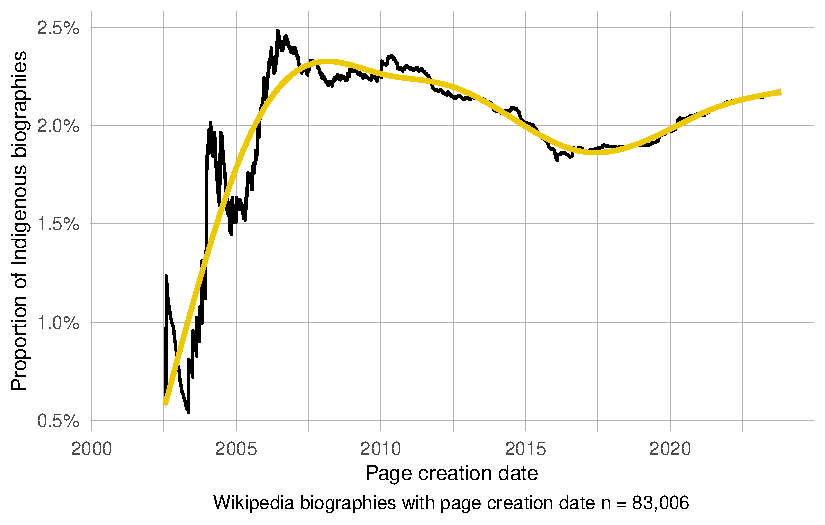
\includegraphics{who-counts_files/figure-pdf/fig-indigenous-growth-wikipedia-1.pdf}

}

\caption{\label{fig-indigenous-growth-wikipedia}In recent years, the
proportion of Indigenous biographies may have started to grow.}

\end{figure}

The situation in Wikidata is made simple by the fact that it has no
system for ethnic or national classification. There are two main markers
of indigenity for Australians in Wikidata:

\begin{enumerate}
\def\labelenumi{\arabic{enumi}.}
\tightlist
\item
  A person's `description' may mention their indigeneity. For example,
  \href{https://www.wikidata.org/w/index.php?title=Q817828\&oldid=1617736683}{Bennelong}
  is described as an `Eora interlocutor with the British in Australia
  and the United Kingdom'. To obtain an estimate of Indigenous
  Australians in the Wikidata data, we have used the crude method of
  seraching for known keywords, including `indigneous', `aboriginal' and
  `eora', then scanning the results by eye to exclude false positives
  (for example \href{}{Judith Wright}, who is described as an
  `Indigenous rights activist' on Wikidata). \textbf{TODO: Kelly, I
  think we need to do this again using the additional 18000 records from
  Category:Australian People}
\item
  A person may be linked to a record in the
  \href{https://ia.anu.edu.au/}{Indigenous Australia} database
  (\href{https://www.wikidata.org/wiki/Property:P9246}{P9246}). At the
  time of writing, the Indigenous Australia database contains
  \href{https://ia.anu.edu.au/biographies/name/}{973 entries} for
  Indigenous Australians. Of these 973, 304 have been linked to a
  Wikidata item.
\end{enumerate}

\hypertarget{historical-period}{%
\section{Historical period}\label{historical-period}}

\begin{itemize}
\tightlist
\item
  size in bytes
\item
  pageviews
\item
  article ratings
\item
  number of edits
\end{itemize}

\emph{TODO}: Dig into category graph to explore gender and indigeneity.

\hypertarget{conclusion-beyond-bias}{%
\chapter{Conclusion: beyond bias}\label{conclusion-beyond-bias}}

TODO

\hypertarget{refs}{}
\begin{CSLReferences}{1}{0}
\leavevmode\vadjust pre{\hypertarget{ref-mandiberg_wikipedias_2023}{}}%
Mandiberg, Michael. 2023. {``Wikipedia's {Race} and {Ethnicity} {Gap}
and the {Unverifiability} of {Whiteness}.''} \emph{Social Text} 41 (1
(154)): 21--46. \url{https://doi.org/10.1215/01642472-10174954}.

\leavevmode\vadjust pre{\hypertarget{ref-weathington_queer_2023}{}}%
Weathington, Katy, and Jed R. Brubaker. 2023. {``Queer {Identities},
{Normative} {Databases}: {Challenges} to {Capturing} {Queerness} {On}
{Wikidata}.''} \emph{Proceedings of the ACM on Human-Computer
Interaction} 7 (CSCW1): 84:1--26. \url{https://doi.org/10.1145/3579517}.

\end{CSLReferences}



\end{document}
